\documentclass[12pt]{article}

\usepackage[a4paper,margin=1in]{geometry}
\usepackage{hyperref}
\usepackage{graphicx}
\usepackage{listings}
\usepackage{color}

\title{CI/CD Pipeline for a Containerized Java Calculator}
\author{Harsha Chigurupati}
\date{\today}

\begin{document}

\maketitle

\tableofcontents

\newpage
\section{Introduction}

Modern software systems are rarely developed or deployed in isolation. 
Instead, they rely on a coordinated ecosystem of tools that automate 
building, testing, packaging, and deployment. The discipline that 
orchestrates these processes is commonly referred to as DevOps. 
DevOps integrates development and operational practices in order to 
facilitate continuous integration and continuous deployment (CI/CD), 
thereby improving both the reliability and velocity of software delivery.

The objective of this project is to construct a minimal yet functional 
CI/CD pipeline for a command-line scientific calculator implemented in Java. 
The pipeline automates compilation, testing, containerization, and deployment 
through a sequence of interconnected tools.

The primary technologies employed in this project are:

\begin{itemize}
\item \textbf{GitHub} – A distributed version control platform used for 
source code hosting and collaboration. It serves as the canonical 
repository for the calculator application's source code.

\item \textbf{Jenkins} – An open-source automation server responsible for 
executing the CI/CD pipeline. Jenkins retrieves the source code from GitHub, 
runs automated tests, builds the project, and orchestrates subsequent steps.

\item \textbf{Docker} – A containerization platform used to package the 
calculator application and its runtime environment into a portable container image.

\item \textbf{Docker Hub} – A container registry used to store and distribute 
Docker images. The built image is pushed to Docker Hub and later retrieved 
during deployment.

\item \textbf{Ansible} – A configuration management and automation tool used 
to provision the deployment environment and execute container-based deployment tasks.
\end{itemize}

The combination of these tools establishes a streamlined pipeline that 
automatically transforms source code into a deployable application.

\bigskip

The project repositories are available at:

\begin{itemize}
\item GitHub Repository: \\
\texttt{https://github.com/VenerableHarsha/Miniproject-calculator.git}

\item Docker Hub Image Repository: \\
\texttt{https://hub.docker.com/repository/docker/venerableharsha/calculator-app/general}
\end{itemize}
\section{CI/CD Pipeline with Jenkins}

Jenkins functions as the central orchestration engine of the pipeline. 
Upon receiving updates from the GitHub repository, Jenkins initiates a 
series of automated stages defined in the \texttt{Jenkinsfile}. 
These stages collectively perform compilation, testing, container image 
construction, and deployment.

The pipeline consists of the following stages:

\begin{itemize}
\item \textbf{Source Retrieval} – Jenkins clones the calculator repository 
from GitHub using the Git SCM plugin.

\item \textbf{Build and Compilation} – The project is compiled using 
Apache Maven. Maven resolves dependencies and produces a runnable JAR file.

\item \textbf{Testing} – Unit tests implemented with JUnit are executed. 
This stage ensures that the calculator's mathematical operations behave 
correctly prior to containerization.

\item \textbf{Container Image Construction} – Docker is used to construct 
a container image containing the compiled calculator application.

\item \textbf{Image Publication} – The resulting Docker image is pushed to 
Docker Hub, making it accessible for deployment.

\item \textbf{Deployment} – Ansible is invoked to provision the deployment 
environment and launch the calculator container.

\item \textbf{Post-Action} - Jenkins triggers an email notification to notify upon the build success or failure
\end{itemize}
\section{Containerization with Docker}

Docker is employed to encapsulate the application and its runtime 
environment within a container image. This approach ensures that the 
application executes consistently across different environments.

The Dockerfile defines the steps required to build the container image. 
The base image provides a lightweight Java runtime environment, upon 
which the compiled calculator application is placed.

Once constructed, the image is tagged and pushed to Docker Hub. 
This enables the deployment stage to retrieve the image from a centralized 
registry rather than relying on locally built artifacts.
\subsection{Jenkins Pipeline Configuration}

After installing Jenkins, a new pipeline job was created to automate the
build and deployment process for the calculator application.

From the Jenkins dashboard, the option \textbf{New Item} was selected and a
new project was created using the \textbf{Pipeline} project type. This option
allows Jenkins to execute build instructions defined in a \texttt{Jenkinsfile}
stored in the project's source repository.

The pipeline job was configured to retrieve the project source code directly
from the GitHub repository. The repository URL was provided in the pipeline
configuration so that Jenkins could clone the project during execution.

Additionally, the pipeline definition was configured to use the
\textbf{Pipeline Script from SCM} option. This allows Jenkins to automatically
load the pipeline instructions from the \texttt{Jenkinsfile} present in the
repository.

The following screenshots illustrate the configuration steps used to create
the Jenkins pipeline job.

\begin{figure}[h]
\centering

\includegraphics[width=0.9\linewidth]{images/SCM.png}
\caption{Creating a new Jenkins pipeline project}
\end{figure}

\begin{figure}[h]
\centering
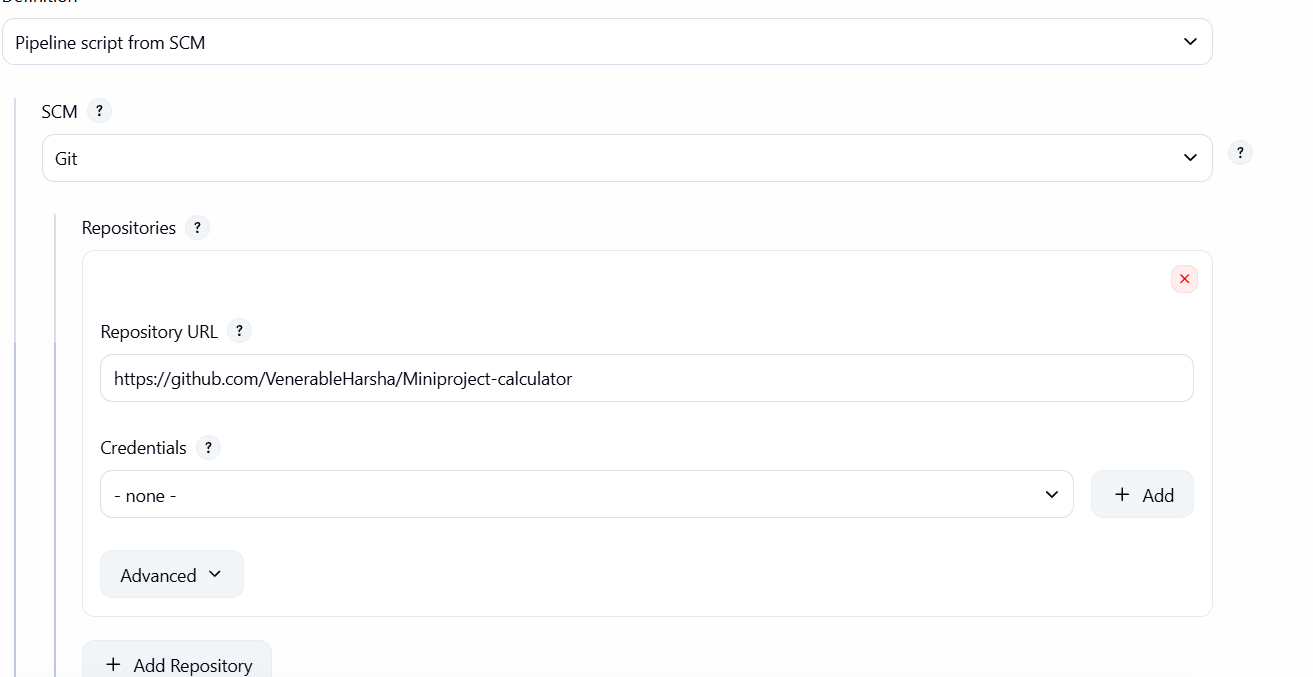
\includegraphics[width=0.9\linewidth]{images/github.png}
\caption{Jenkins pipeline configuration using the GitHub repository}
\end{figure}

\begin{figure}[h]
\centering
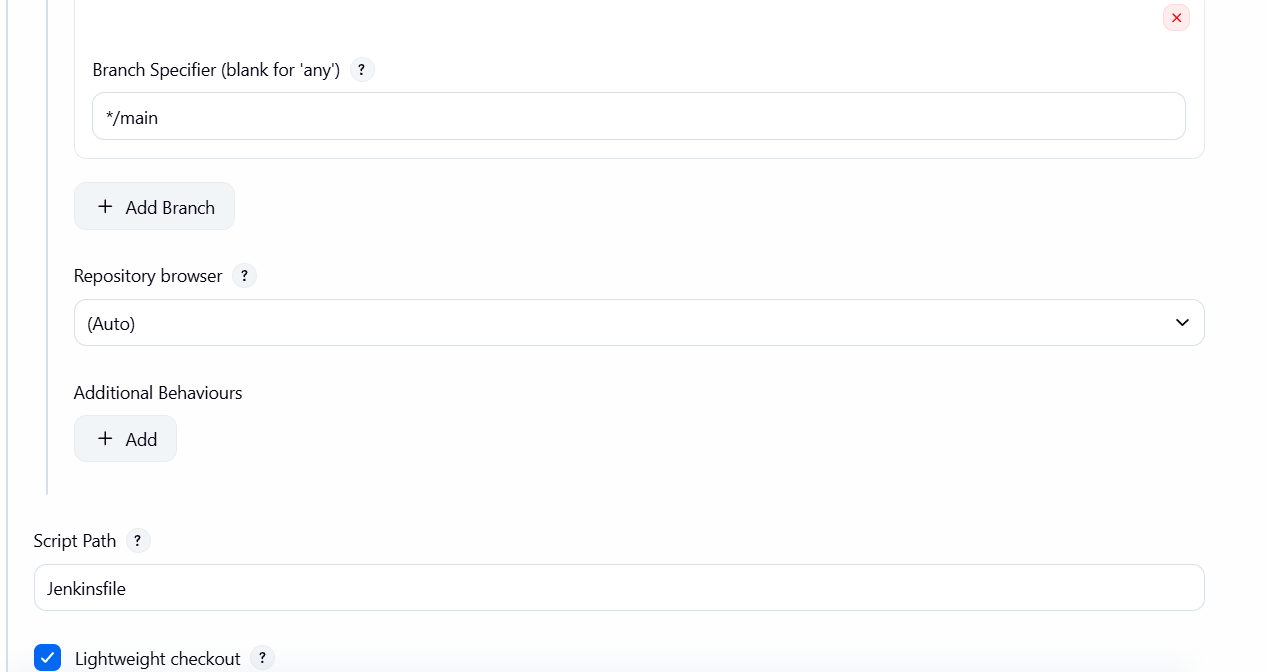
\includegraphics[width=0.9\linewidth]{images/branch.png}
\caption{Pipeline configured to use Jenkinsfile from the source repository}
\end{figure}

\section{Deployment Automation with Ansible}

Ansible is utilized to automate the provisioning of the deployment 
environment and the execution of container operations.

The \texttt{inventory.ini} file specifies the target host for deployment. 
In this project, the host corresponds to the local deployment environment 
managed within the Docker ecosystem.

The \texttt{deploy.yml} playbook contains the automation logic. 
Its responsibilities include:

\begin{itemize}
\item Ensuring that the deployment container exists and remains active.
\item Pulling the latest calculator image from Docker Hub.
\item Launching the calculator container within the deployment environment.
\end{itemize}

Through this mechanism, the deployment process becomes reproducible and 
consistent, eliminating the need for manual configuration.
\section{System Architecture}

The complete CI/CD workflow integrates several tools into a coherent 
pipeline. Source code modifications trigger automated build and deployment 
processes that ultimately produce a runnable containerized application.

The high-level architecture of the system is illustrated using the 
PlantUML diagram below.
\begin{figure}[htbp]
    \centering
    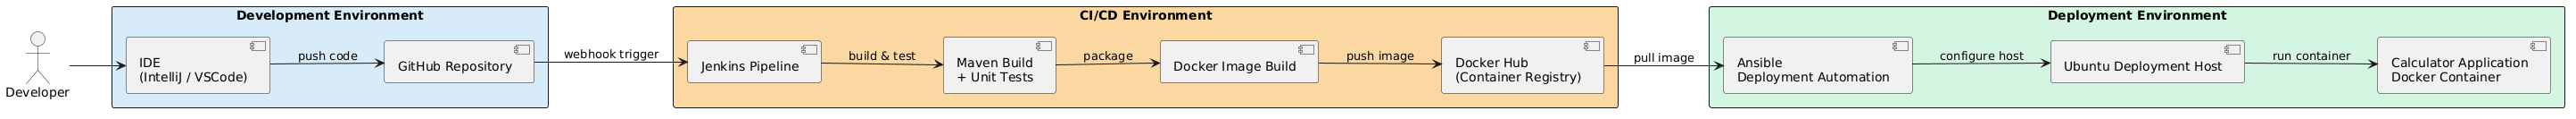
\includegraphics[width=1.0\linewidth]{images/architecture.png}
    \caption{Architecture diagram }
    \label{fig:label_name}
\end{figure}
\subsection{Development and Execution Environment}

All development and pipeline execution in this project was performed on a
single local workstation using Windows and Windows Subsystem for Linux (WSL).

The development workflow was divided across multiple environments:

\begin{itemize}

\item \textbf{Development Environment (Windows)} \\
The calculator application was developed using IntelliJ IDEA running on
Windows. Source code editing, project structure management, and local testing
were performed within this environment.

\item \textbf{Build and CI Environment (WSL Ubuntu)} \\
Jenkins, Docker, Maven, and Ansible were installed inside a WSL Ubuntu
environment. This Linux environment served as the CI/CD execution platform
responsible for compiling the application, running tests, building container
images, and executing deployment automation.

\item \textbf{Deployment Environment (Fresh Ubuntu Container)} \\
For deployment simulation, a fresh Ubuntu container was created to act as the
target host. This container represented a clean runtime environment into which
the application container would be deployed.

\end{itemize}

To reduce resource overhead, a separate Docker daemon was not launched inside
the deployment container. Instead, the container was configured to use the
Docker service already running in the WSL host environment. This approach
allowed the deployment process to interact with Docker without running nested
container services.
\subsection{Exposing the Jenkins Server using ngrok}

Since Jenkins was running locally inside the WSL Ubuntu environment, it was not
directly accessible from external services such as GitHub. However, the CI/CD
pipeline relies on GitHub webhooks to trigger builds whenever changes are
pushed to the repository.

To enable GitHub to communicate with the locally running Jenkins server,
\textbf{ngrok} was used to expose the Jenkins HTTP endpoint to the public
internet.

Ngrok creates a secure tunnel from a public URL to a local service. In this
project, the Jenkins server running on port 8080 was exposed using the
following command:

\begin{verbatim}
ngrok http 8080
\end{verbatim}

This command generated a temporary public URL that forwarded incoming HTTP
requests to the Jenkins server running on the local machine.

The generated ngrok URL was then used to configure the GitHub webhook so that
any push event in the repository would trigger the Jenkins pipeline.

Through this mechanism, GitHub was able to notify Jenkins of repository updates
even though Jenkins was running within a local development environment.

A screenshot of the active ngrok tunnel is shown below.

\begin{figure}[h]
\centering
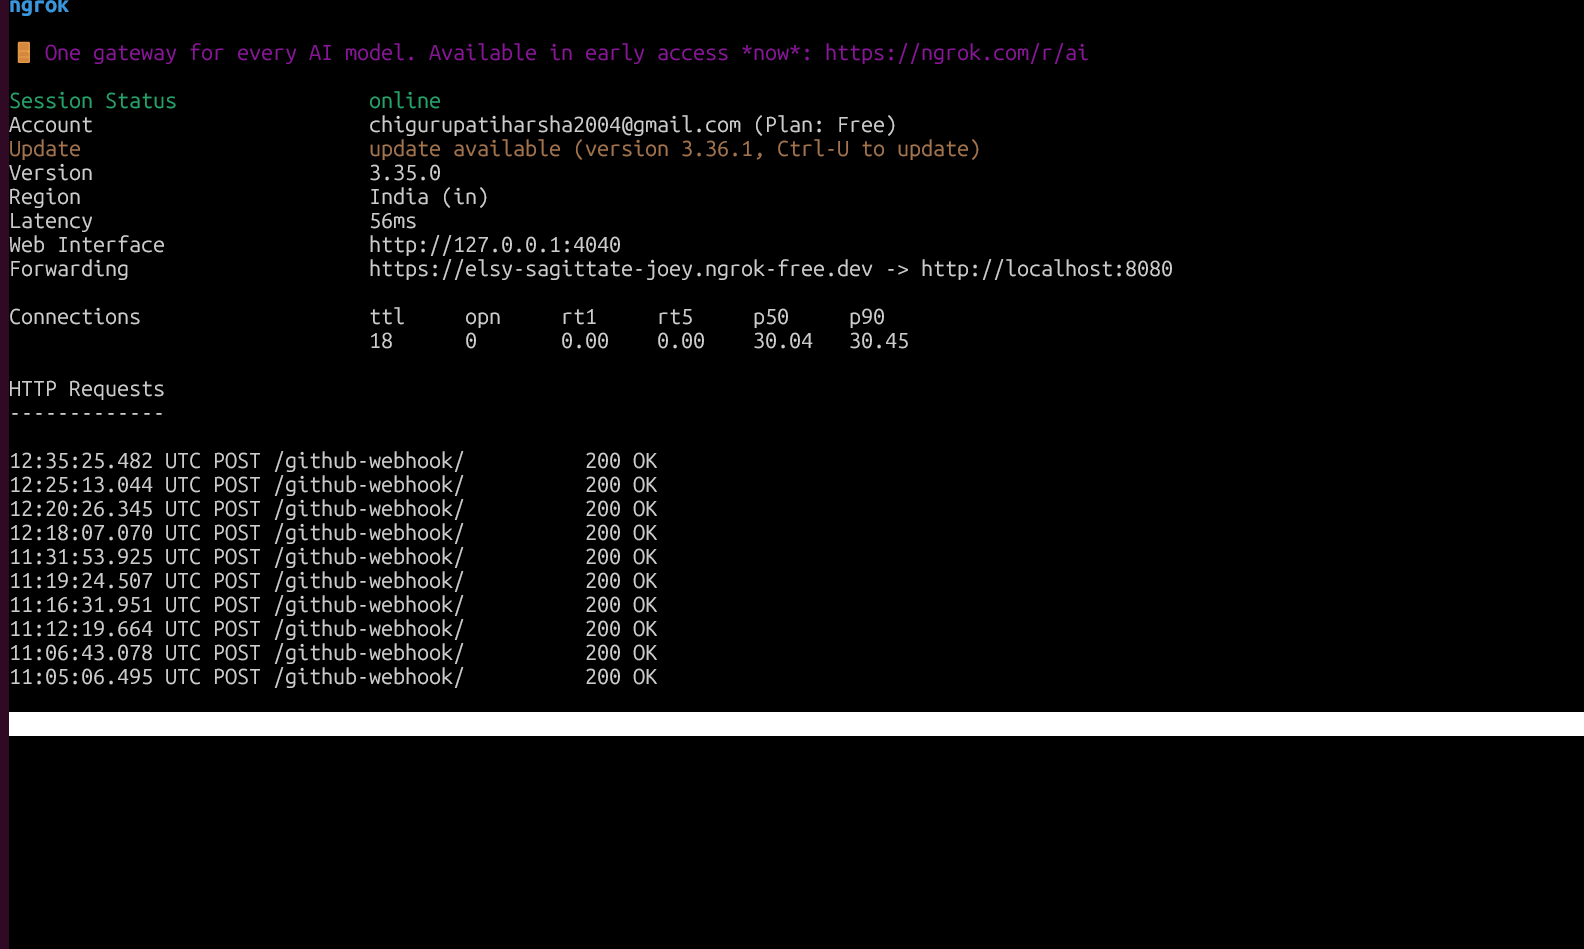
\includegraphics[width=0.9\linewidth]{images/ngrok.png}
\caption{Running Ngrok that catches webhooks}
\end{figure}
\subsection{Jenkins Pipeline Execution Stages}

The Jenkins pipeline is defined through a declarative configuration file
known as the \texttt{Jenkinsfile}. This file specifies a sequence of stages
that are executed whenever the pipeline is triggered.

Each stage performs a specific task in transforming the source code into a
deployed containerized application. The following sections describe the
function of each stage in the pipeline.

\subsubsection{Build Stage}

The pipeline begins with the build stage. In this step Jenkins navigates to the
project directory containing the calculator source code.

The Apache Maven build system is then invoked to compile the Java source files.
During this process Maven performs several tasks automatically:

\begin{itemize}

\item Downloads any required dependencies from the Maven Central repository
if they are not already present locally.

\item Compiles all Java source files into bytecode.

\item Verifies that the project structure conforms to the Maven build model.

\end{itemize}

At the end of this stage the project has been successfully compiled but has not
yet been packaged into a runnable artifact.

\subsubsection{Test Execution Stage}

After compilation completes successfully, the pipeline proceeds to the testing
stage. In this stage Maven executes the project's automated unit tests.

The tests validate the correctness of the calculator's mathematical operations
such as addition, subtraction, multiplication, and division. Running these
tests before packaging ensures that only verified code proceeds further in the
pipeline.

If any test fails, the Jenkins pipeline immediately terminates and the build
is marked as failed. This prevents defective code from being packaged or
deployed.

If all tests pass successfully, Jenkins advances to the packaging stage.

\subsubsection{Application Packaging Stage}

Once testing has completed successfully, the pipeline packages the compiled
application.

Maven produces a runnable Java archive (JAR file) containing the compiled
calculator application and the metadata required to execute it. This artifact
serves as the executable component that will later be placed inside the Docker
container image.

The packaging step ensures that the application exists as a single portable
binary which can be easily transferred between environments.


\subsubsection{Docker Image Construction}

After the application has been packaged, the pipeline constructs a Docker
container image.

During this step Docker reads the instructions contained in the project's
Dockerfile. The Dockerfile defines the base runtime environment, copies the
packaged application artifact into the container, and specifies the command
required to launch the calculator program.

The result of this process is a Docker image containing the calculator
application together with the Java runtime environment necessary to execute it.

This image is tagged using a version identifier so that it can later be
published to a container registry.

\subsubsection{Docker Image Publication}

Once the container image has been built locally, the pipeline publishes the
image to Docker Hub.

To perform this operation Jenkins authenticates with Docker Hub using stored
credentials configured within the Jenkins credential manager. These
credentials allow Jenkins to securely log into the registry without exposing
authentication information in the pipeline configuration.

After authentication, the image is pushed to Docker Hub. This step makes the
container image available to external systems and deployment environments.

Using a centralized registry ensures that deployment processes retrieve a
consistent and verified version of the application.

\subsubsection{Deployment using Ansible}

The final stage of the pipeline performs automated deployment using Ansible.

In this stage Jenkins invokes an Ansible playbook which contains the
instructions required to deploy the application container. The playbook
interacts with the deployment environment specified in the
\texttt{inventory.ini} configuration file.

During deployment the playbook performs the following actions:

\begin{itemize}

\item Connects to the target deployment host.

\item Pulls the latest calculator container image from Docker Hub.

\item Starts a new Docker container running the calculator application.

\end{itemize}

The deployment process therefore retrieves the container image produced by the
pipeline and launches it in a fresh runtime environment. This simulates the
behavior of a production deployment pipeline where container images are
distributed and executed across remote hosts.

Finally we get an email notification, for this project I have used dummy email as sender and a non-existent email as reciever.

\begin{figure}[h]
\centering
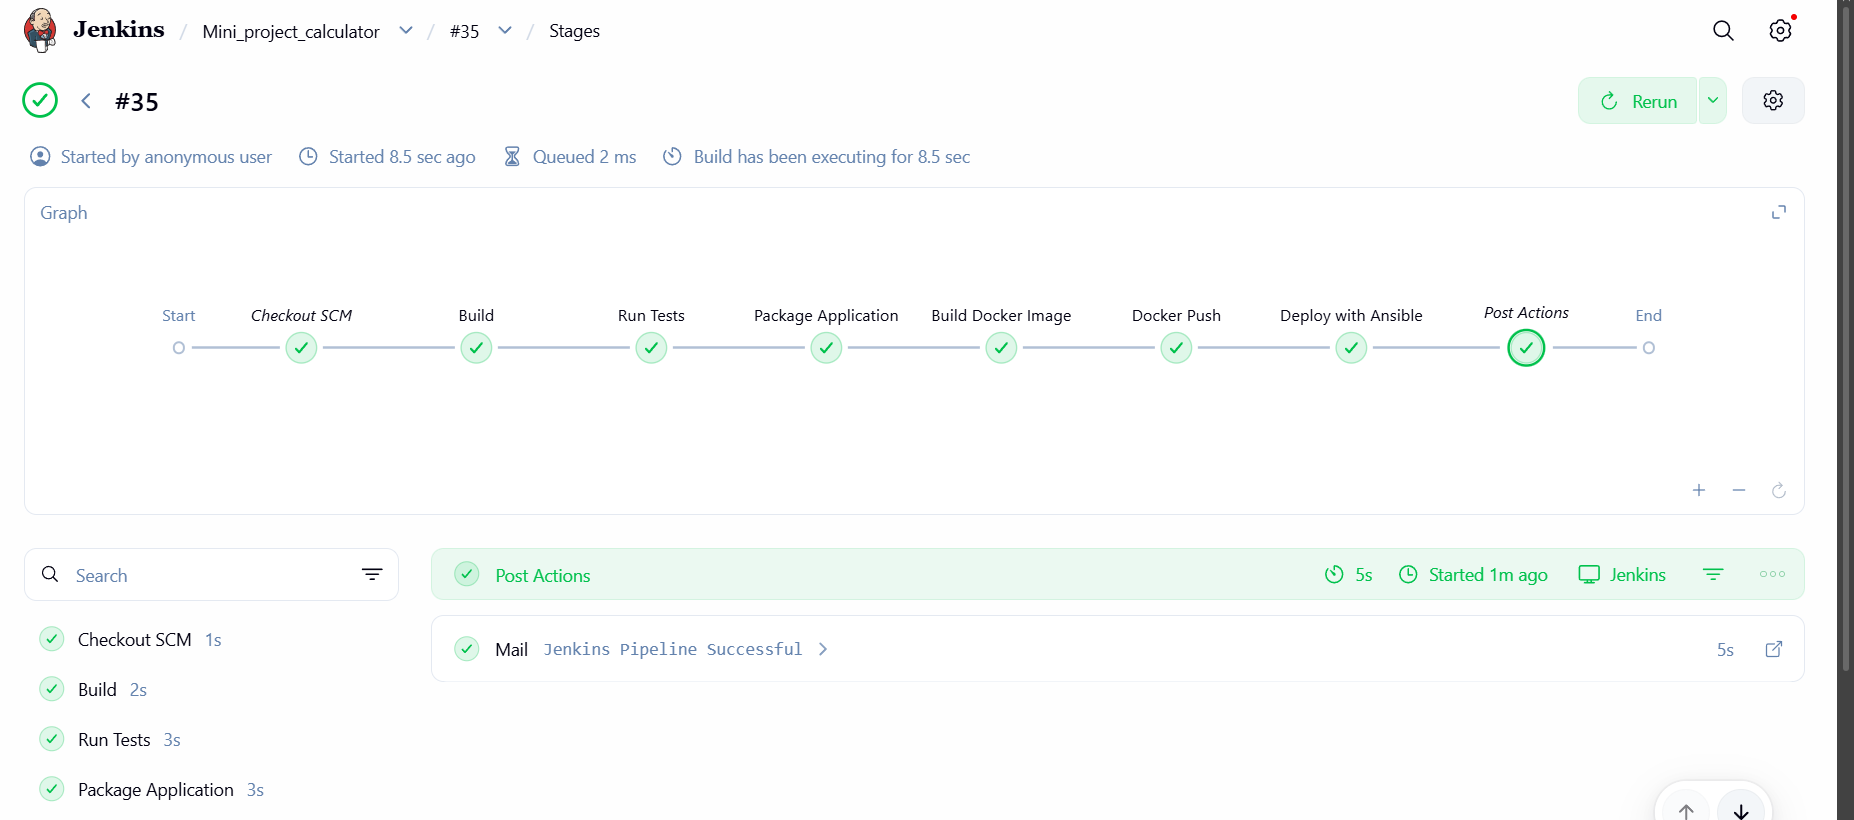
\includegraphics[width=0.9\linewidth]{images/successful.png}
\caption{A successful pipeline build}
\end{figure}
\begin{figure}[h]
\centering
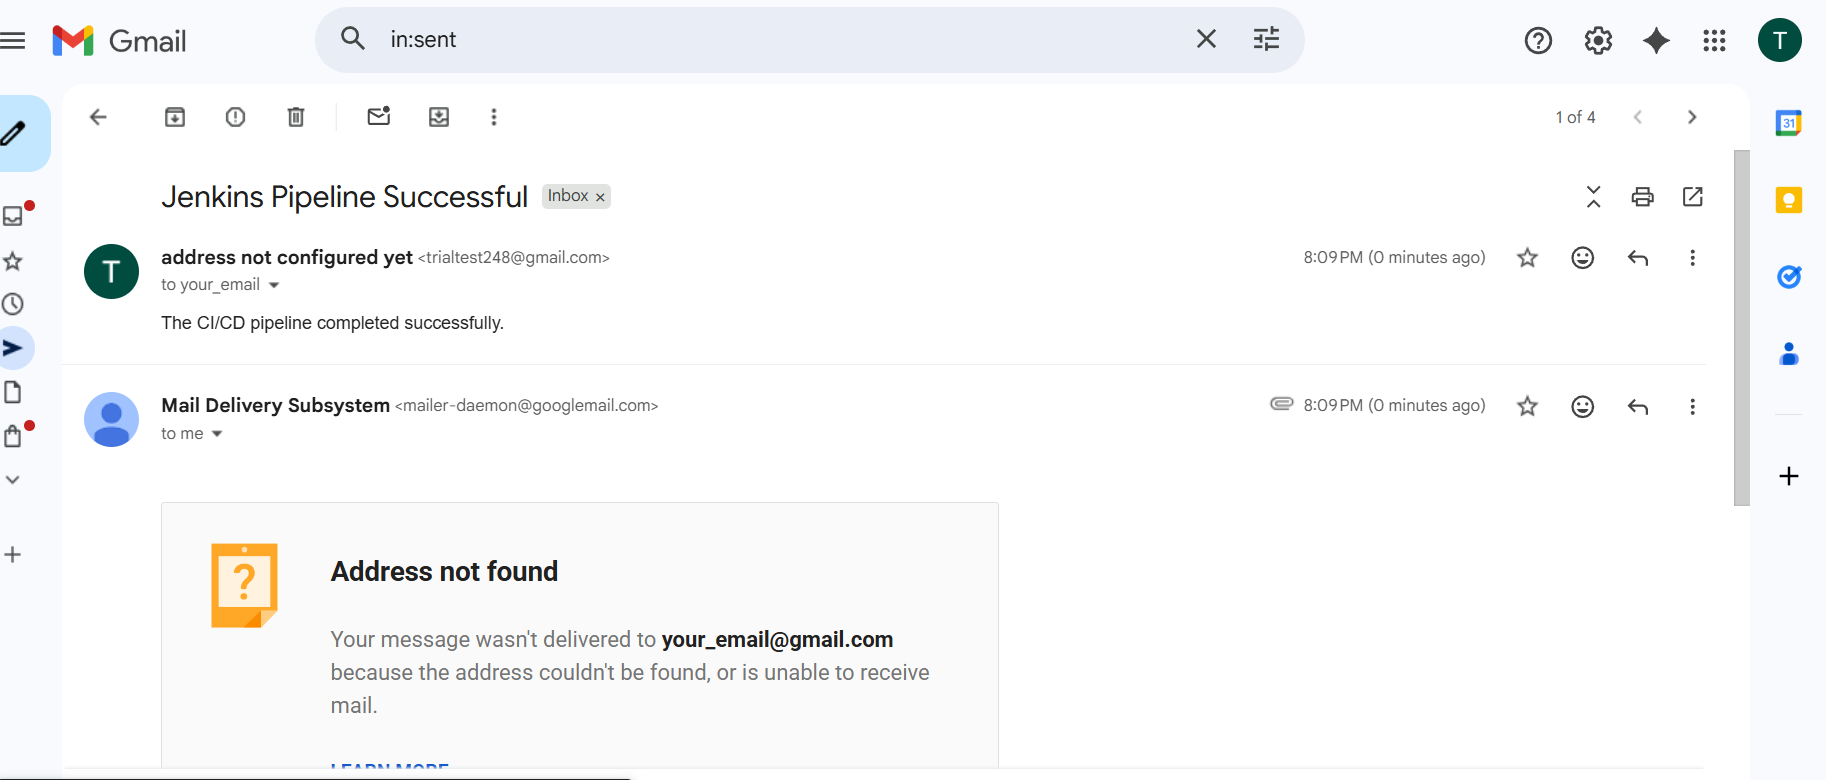
\includegraphics[width=0.9\linewidth]{images/email.png}
\caption{Example email notification}
\end{figure}
\begin{figure}[htbp]
    \centering
    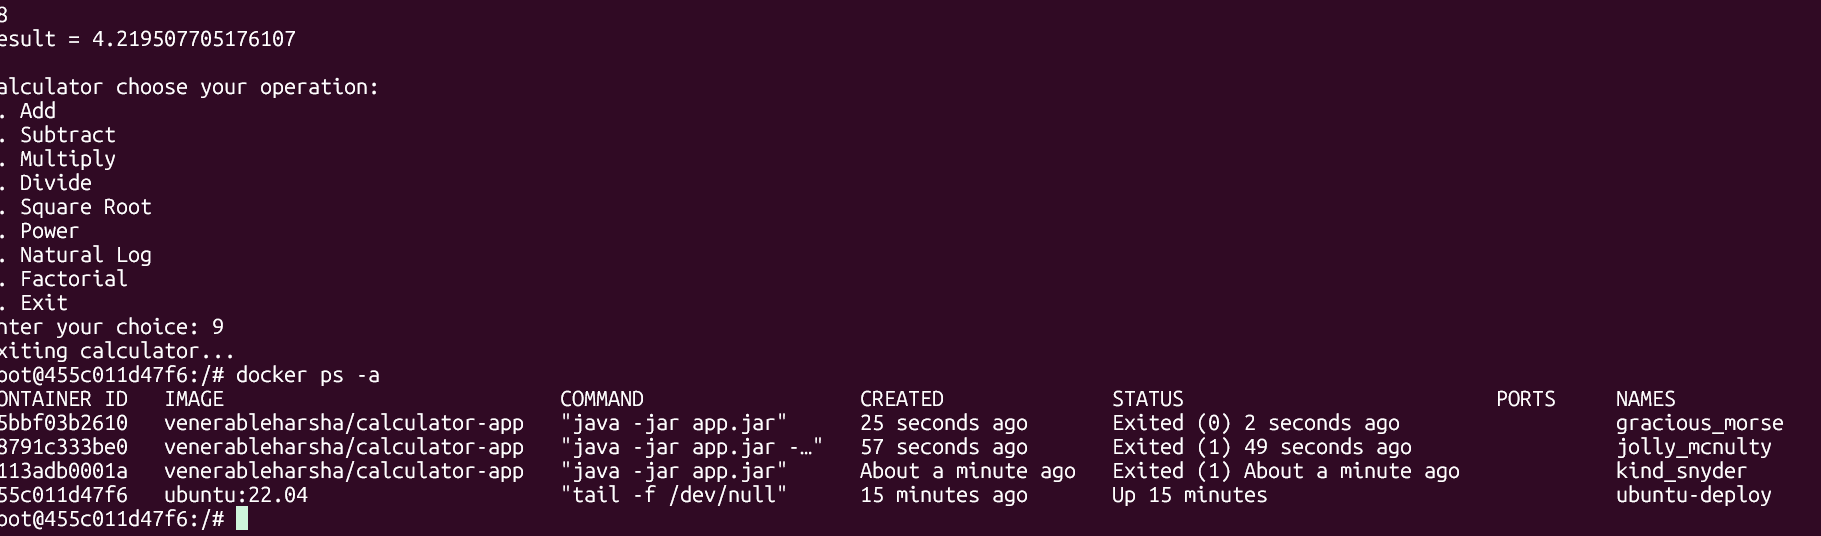
\includegraphics[width=1.0\linewidth]{images/docker.png}
    \caption{Docker images once deployed}
    \label{fig:label_name}
\end{figure}
\begin{figure}[htbp]
    \centering
    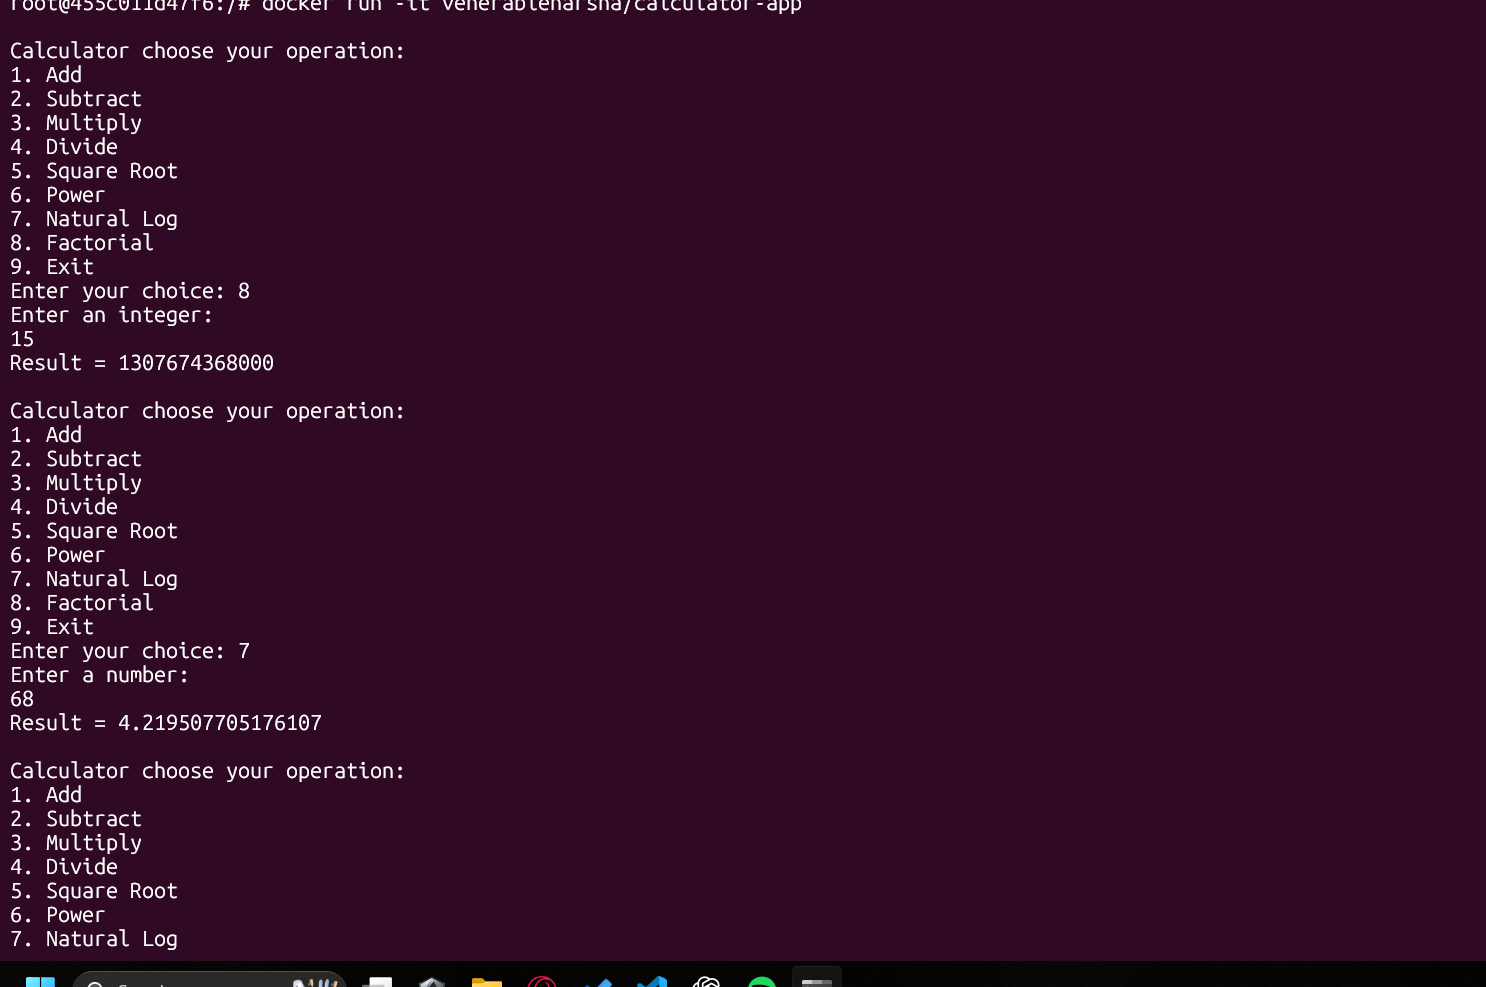
\includegraphics[width=1.0\linewidth]{images/calculator.png}
    \caption{Runnning calculator}
    \label{fig:label_name}
\end{figure}


\section{Conclusion}

This project demonstrates the construction of a lightweight yet 
fully functional CI/CD pipeline integrating several widely adopted 
DevOps technologies. By combining version control, automated builds, 
containerization, and configuration management, the pipeline ensures 
that application updates can be propagated from source code to deployment 
with minimal manual intervention.

The architecture illustrates how modern software delivery pipelines 
leverage automation to improve reliability, reproducibility, and 
operational efficiency.
\section{References}

\begin{itemize}
\item Docker Documentation – https://docs.docker.com
\item Jenkins Documentation – https://www.jenkins.io/doc/
\item Ansible Documentation – https://docs.ansible.com
\item Maven Documentation – https://maven.apache.org
\end{itemize}
\end{document}